% !TEX program = pdflatex
\documentclass[aspectratio=169, 10pt]{beamer}

% --- PACKAGES ---
\usepackage{amsmath}
\usepackage{amssymb}
\usepackage{booktabs}
\usepackage{siunitx}
\usepackage{tikz}
\usetikzlibrary{arrows.meta, positioning, shapes.geometric, calc, backgrounds, fit, patterns}

% --- COLOR DEFINITIONS ---
\definecolor{Garnet}{HTML}{73000A}
\definecolor{GarnetDark}{HTML}{500007}
\definecolor{Rose}{HTML}{CC2E40}
\definecolor{Atlantic}{HTML}{466A9F}
\definecolor{Congaree}{HTML}{1F414D}
\definecolor{Horseshoe}{HTML}{65780B}
\definecolor{Grass}{HTML}{CED318}
\definecolor{Honeycomb}{HTML}{A49137}
\definecolor{Black90}{HTML}{363636}
\definecolor{Black70}{HTML}{5C5C5C}
\definecolor{Black30}{HTML}{C7C7C7}
\definecolor{Black10}{HTML}{ECECEC}

% --- BEAMER THEME CONFIGURATION ---
\usetheme{default}
\usecolortheme{default}

% Remove navigation symbols
\setbeamertemplate{navigation symbols}{}

% Frame title: sharp Garnet rectangle
\setbeamertemplate{frametitle}{%
  \nointerlineskip
  \begin{beamercolorbox}[wd=\paperwidth,ht=1.0cm,dp=0.3cm]{frametitle}
    \hspace{0.5cm}\insertframetitle
  \end{beamercolorbox}
}

% Block settings: no rounded corners
\setbeamertemplate{blocks}[default]
\setbeamertemplate{itemize items}[square]
\setbeamertemplate{enumerate items}[square]

% Colors
\setbeamercolor{frametitle}{fg=white, bg=Garnet}
\setbeamercolor{title}{fg=white}
\setbeamercolor{author}{fg=white}
\setbeamercolor{date}{fg=white}
\setbeamercolor{normal text}{fg=Black90}
\setbeamercolor{structure}{fg=Garnet}
\setbeamercolor{itemize item}{fg=Garnet}
\setbeamercolor{enumerate item}{fg=Garnet}
\setbeamercolor{block title}{fg=Garnet, bg=Black10}
\setbeamercolor{block body}{fg=Black90, bg=white}
\setbeamercolor{block title alerted}{fg=white, bg=Rose}
\setbeamercolor{block body alerted}{fg=Black90, bg=white}
\setbeamercolor{block title example}{fg=white, bg=Atlantic}
\setbeamercolor{block body example}{fg=Black90, bg=white}

% Footer
\setbeamertemplate{footline}{%
  \leavevmode%
  \hbox{%
    \begin{beamercolorbox}[wd=.5\paperwidth,ht=2.5ex,dp=1ex,left]{author in head/foot}%
      \hspace{0.5cm}AIAA Region II Student Conference 2026
    \end{beamercolorbox}%
    \begin{beamercolorbox}[wd=.3\paperwidth,ht=2.5ex,dp=1ex,center]{title in head/foot}%
      University of South Carolina
    \end{beamercolorbox}%
    \begin{beamercolorbox}[wd=.2\paperwidth,ht=2.5ex,dp=1ex,right]{date in head/foot}%
      \insertframenumber{} / \inserttotalframenumber\hspace{0.5cm}
    \end{beamercolorbox}%
  }%
  \vskip0pt%
}

% Title page
\defbeamertemplate{title page}{custom}[1][]{
  \begin{tikzpicture}[remember picture,overlay]
    \fill[Garnet] (current page.north west) rectangle (current page.south east);
    \node[text=white, text width=0.85\paperwidth, align=center] at (current page.center) {
      {\fontsize{20}{24}\selectfont\bfseries\inserttitle\par}
      \vspace{1.5cm}
      {\fontsize{12}{14}\selectfont\insertauthor\par}
      \vspace{0.5cm}
      {\fontsize{11}{13}\selectfont\insertinstitute\par}
      \vspace{0.5cm}
      {\fontsize{10}{12}\selectfont\insertdate\par}
    };
  \end{tikzpicture}
}
\setbeamertemplate{title page}[custom]

% Section divider slides
\AtBeginSection[]{
  \begin{frame}[plain]
    \begin{tikzpicture}[remember picture,overlay]
      \fill[Garnet] (current page.north west) rectangle (current page.south east);
      \node[text=white, font=\Huge\bfseries] at (current page.center) {\insertsection};
    \end{tikzpicture}
  \end{frame}
}

% --- METADATA ---
\title{A Multi-Mode Simulation Framework for X-Band Pulse Compression Radar}
\author{J.C. Vaught, D. Cahl, Y. Wang}
\institute{Department of Mechanical Engineering\\University of South Carolina}
\date{AIAA Region II Student Conference\\February 2026}

\begin{document}

% ============================================================
% TITLE SLIDE
% ============================================================
\begin{frame}[plain]
  \titlepage
\end{frame}

% ============================================================
% MOTIVATION
% ============================================================
\begin{frame}
  \frametitle{Motivation: Data Scarcity for Radar-Based Perception}

  \begin{columns}[T]
    \begin{column}{0.48\textwidth}
      \textbf{Problem:}
      \begin{itemize}
        \item Autonomous USVs require robust radar perception
        \item Deep learning models need large labeled datasets
        \item Field data collection is expensive and time-consuming
        \item Small recreational boats produce intermittent, low-RCS returns
        \item Inland waterway clutter is heterogeneous and poorly characterized
      \end{itemize}
    \end{column}

    \begin{column}{0.48\textwidth}
      \textbf{Why X-Band Marine Radar?}
      \begin{itemize}
        \item All-weather, day-night operation
        \item Relevant collision avoidance ranges
        \item COTS units are compact, affordable, field-proven
        \item Complementary to camera/lidar
      \end{itemize}

      \vspace{0.5cm}
      \textbf{Solution:}
      \begin{itemize}
        \item Generate synthetic training data
        \item Multiple abstraction levels for different workflow stages
      \end{itemize}
    \end{column}
  \end{columns}
\end{frame}

% ============================================================
% RELATED WORK
% ============================================================
\begin{frame}
  \frametitle{Related Work and Background}

  \begin{block}{Synthetic Data for Perception}
    \begin{itemize}
      \item Domain randomization effective for camera-based object detection
      \item SAR simulation well-developed, but navigation-band marine radar lags
      \item Sim-to-real transfer remains challenging for radar
    \end{itemize}
  \end{block}

  \begin{block}{Sea Clutter Modeling}
    \begin{itemize}
      \item Compound K-distribution: standard model for X-band sea clutter
      \item Captures heavy-tailed amplitude statistics from Bragg scattering
      \item Ocean models available, but inland waterways poorly characterized
    \end{itemize}
  \end{block}

  \begin{block}{Marine Radar Object Detection}
    \begin{itemize}
      \item Traditional: CFAR processors
      \item Modern: Deep learning (YOLO, Faster R-CNN)
      \item Challenge: Labeled datasets scarce, especially for inland environments
    \end{itemize}
  \end{block}
\end{frame}

% ============================================================
% SYSTEM ARCHITECTURE
% ============================================================
\begin{frame}
  \frametitle{Multi-Mode Framework Architecture}

  \vspace{0.3cm}
  \begin{center}
  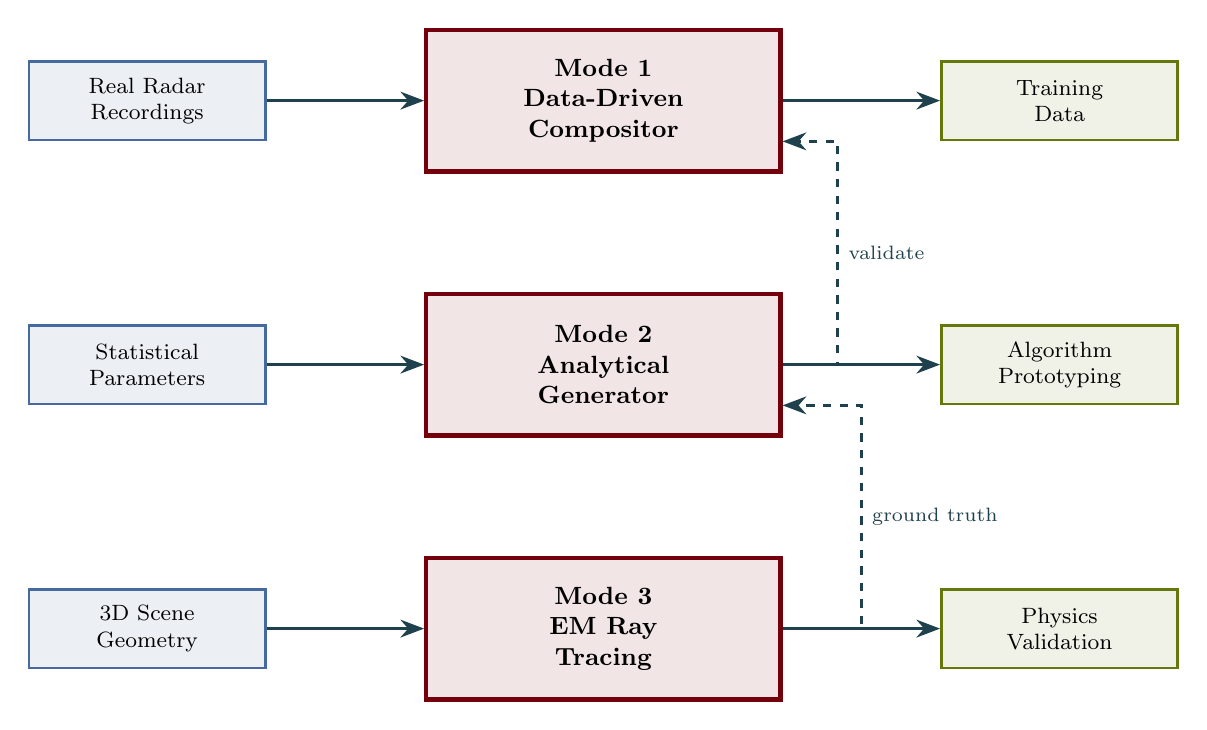
\begin{tikzpicture}[
      node distance=1.2cm and 1.5cm,
      mode/.style={rectangle, draw=Garnet, line width=1.5pt, fill=Garnet!10, minimum width=4.5cm, minimum height=1.8cm, align=center, font=\small\bfseries},
      data/.style={rectangle, draw=Atlantic, line width=1pt, fill=Atlantic!10, minimum width=3cm, minimum height=1cm, align=center, font=\footnotesize},
      output/.style={rectangle, draw=Horseshoe, line width=1pt, fill=Horseshoe!10, minimum width=3cm, minimum height=1cm, align=center, font=\footnotesize},
      arrow/.style={-{Stealth[length=3mm]}, line width=1.2pt, Congaree},
      dasharrow/.style={-{Stealth[length=3mm]}, line width=1.2pt, Congaree, dashed},
  ]

  % Modes
  \node[mode] (m1) {Mode 1\\Data-Driven\\Compositor};
  \node[mode, below=1.5cm of m1] (m2) {Mode 2\\Analytical\\Generator};
  \node[mode, below=1.5cm of m2] (m3) {Mode 3\\EM Ray\\Tracing};

  % Inputs
  \node[data, left=2cm of m1] (real) {Real Radar\\Recordings};
  \node[data, left=2cm of m2] (params) {Statistical\\Parameters};
  \node[data, left=2cm of m3] (scene) {3D Scene\\Geometry};

  % Outputs
  \node[output, right=2cm of m1] (train) {Training\\Data};
  \node[output, right=2cm of m2] (proto) {Algorithm\\Prototyping};
  \node[output, right=2cm of m3] (valid) {Physics\\Validation};

  % Arrows
  \draw[arrow] (real) -- (m1);
  \draw[arrow] (params) -- (m2);
  \draw[arrow] (scene) -- (m3);
  \draw[arrow] (m1) -- (train);
  \draw[arrow] (m2) -- (proto);
  \draw[arrow] (m3) -- (valid);

  % Cross-mode validation arrows
  \draw[dasharrow] (m2.east) -- ++(0.7,0) |- node[right, pos=0.25, font=\scriptsize, text=Congaree]{validate} (m1.east |- train.south);
  \draw[dasharrow] (m3.east) -- ++(1,0) |- node[right, pos=0.25, font=\scriptsize, text=Congaree]{ground truth} (m2.east |- proto.south);

  \end{tikzpicture}
  \end{center}

  \vspace{0.2cm}
  \begin{itemize}
    \item Modes ordered by workflow utility, not physics resolution
    \item Shared world model ensures cross-mode validation
  \end{itemize}
\end{frame}

% ============================================================
% MODE 1
% ============================================================
\begin{frame}
  \frametitle{Mode 1: Data-Driven Compositor}

  \textbf{Approach:} Blend synthetic target signatures into real radar recordings

  \vspace{0.3cm}
  \begin{center}
  \begin{tikzpicture}[
      step/.style={rectangle, draw=Garnet, line width=1pt, fill=Black10, minimum width=2.2cm, minimum height=1cm, align=center, font=\scriptsize},
      arrow/.style={-{Stealth[length=2mm]}, line width=1pt, Congaree},
  ]

  \node[step] (s1) {1. Background\\Selection};
  \node[step, right=0.3cm of s1] (s2) {2. Target\\Signature\\Generation};
  \node[step, right=0.3cm of s2] (s3) {3. Amplitude\\Matching};
  \node[step, right=0.3cm of s3] (s4) {4. Insertion\\and Blending};
  \node[step, right=0.3cm of s4] (s5) {5. Label\\Generation};

  \draw[arrow] (s1) -- (s2);
  \draw[arrow] (s2) -- (s3);
  \draw[arrow] (s3) -- (s4);
  \draw[arrow] (s4) -- (s5);

  \end{tikzpicture}
  \end{center}

  \vspace{0.5cm}
  \textbf{Key Advantages:}
  \begin{itemize}
    \item Inherits authentic sensor noise, clutter texture, and artifacts
    \item Minimal sim-to-real gap
    \item Complete control over target placement and labeling
  \end{itemize}

  \vspace{0.3cm}
  \textbf{Environmental Augmentation:}
  \begin{itemize}
    \item Radar interference patterns extracted from Charleston Harbor
    \item Rain clutter textures from weather events
    \item Exposes detector to degraded conditions without additional field collections
  \end{itemize}
\end{frame}

% ============================================================
% MODE 2
% ============================================================
\begin{frame}
  \frametitle{Mode 2: Analytical Generator}

  \textbf{Approach:} Synthesize complete radar frames from parametric statistical models

  \begin{columns}[T]
    \begin{column}{0.48\textwidth}
      \textbf{Clutter Model:}\\
      Compound K-distribution

      \vspace{0.2cm}
      \begin{equation*}
        f(x) = \frac{4}{\Gamma(\nu)} \left(\frac{\nu}{P_c}\right)^{\!\frac{\nu+1}{2}} x^{\nu}\, K_{\nu-1}\!\left(2\sqrt{\frac{\nu\, x^2}{P_c}}\right)
      \end{equation*}

      \begin{itemize}
        \item $\nu$: shape parameter (tail behavior)
        \item $P_c$: mean clutter power
        \item Small $\nu$ = heavier tails, spikier clutter
        \item Inland lakes: large $\nu$ (approaching Rayleigh)
      \end{itemize}
    \end{column}

    \begin{column}{0.48\textwidth}
      \textbf{Target Model:}\\
      Fluctuating point scatterers, Swerling I distribution

      \vspace{0.2cm}
      Radar equation:
      \begin{equation*}
        P_r = \frac{P_t\, G^2\, \lambda^2\, \sigma}{(4\pi)^3\, R^4\, L}
      \end{equation*}

      \vspace{0.3cm}
      \textbf{Frame Synthesis:}
      \begin{enumerate}
        \item Draw clutter realization from K-distribution
        \item Add target returns with Swerling RCS
        \item Apply log-detection
        \item Add thermal noise and interference
      \end{enumerate}
    \end{column}
  \end{columns}

  \vspace{0.3cm}
  \textbf{Purpose:} Rapid algorithm prototyping without requiring real data
\end{frame}

% ============================================================
% MODE 3
% ============================================================
\begin{frame}
  \frametitle{Mode 3: EM Ray Tracing}

  \textbf{Approach:} Shooting-and-bouncing-rays (SBR) for pulse-level EM simulation

  \begin{columns}[T]
    \begin{column}{0.48\textwidth}
      \textbf{Architecture:}
      \begin{enumerate}
        \item Launch rays from radar antenna (beam pattern)
        \item Propagate through scene, intersect water surface and targets
        \item Generate reflected/scattered rays (material-dependent)
        \item Coherently sum rays returning to aperture
        \item Match-filter (pulse compression) and log-detect
      \end{enumerate}

      \vspace{0.3cm}
      \textbf{Water Surface:}
      \begin{itemize}
        \item Time-varying mesh from wind-driven wave spectrum
        \item Multipath between direct and specular reflection paths
      \end{itemize}
    \end{column}

    \begin{column}{0.48\textwidth}
      \textbf{Purpose:}
      \begin{itemize}
        \item Physics-grounded reference data
        \item Validate assumptions in Modes 1 and 2
        \item Study multipath, scattering, and clutter mechanisms
      \end{itemize}

      \vspace{0.3cm}
      \textbf{Current Status:}
      \begin{itemize}
        \item Functional for canonical scenarios (single targets, flat/perturbed water)
        \item Preliminary validation against two-ray (Lloyd's mirror) model
        \item Extension to complex scenes (shorelines, docks, vegetation) ongoing
      \end{itemize}
    \end{column}
  \end{columns}
\end{frame}

% ============================================================
% SENSOR CHARACTERIZATION
% ============================================================
\begin{frame}
  \frametitle{Sensor Platform: Furuno DRS4D NXT}

  \begin{columns}[T]
    \begin{column}{0.55\textwidth}
      \begin{table}
        \centering
        \small
        \begin{tabular}{@{}ll@{}}
          \toprule
          \textbf{Parameter} & \textbf{Value} \\
          \midrule
          Transmitter & Solid-state, pulse compression \\
          Frequency & 9.38--9.44 GHz (X-band) \\
          Output power & 100 W \\
          Modulation & LFM chirp / unmodulated \\
          Chirp width & 5.0--18 $\mu$s (range-dependent) \\
          Range resolution & $\sim$20 m \\
          Horiz.\ beamwidth & 3.9$^{\circ}$ (RezBoost disabled) \\
          Vert.\ beamwidth & 22--25$^{\circ}$ \\
          Rotation rate & 24 / 36 / 48 RPM \\
          PRF & 700--1100 Hz \\
          Azimuth quant. & 8{,}192 spokes/rev \\
          Radome diameter & 610 mm (24 in) \\
          \bottomrule
        \end{tabular}
      \end{table}
    \end{column}

    \begin{column}{0.4\textwidth}
      \textbf{Key Features:}
      \begin{itemize}
        \item Doppler-capable
        \item RezBoost disabled to preserve weak returns
        \item UDP multicast spoke-format intensity data
        \item Log-detected, non-coherent (no I/Q)
      \end{itemize}

      \vspace{0.3cm}
      \textbf{Target RCS Estimates:}
      \begin{itemize}
        \item Fiberglass boats: 0.5--20 m$^2$
        \item Aluminum boats/buoys: 1--50 m$^2$
      \end{itemize}
    \end{column}
  \end{columns}
\end{frame}

% ============================================================
% DATA COLLECTION
% ============================================================
\begin{frame}
  \frametitle{Data Collection Campaign}

  \begin{columns}[T]
    \begin{column}{0.48\textwidth}
      \textbf{Locations:}
      \begin{itemize}
        \item Lake Murray, SC
        \item Lake Greenwood, SC
        \item Charleston Harbor, SC
      \end{itemize}

      \vspace{0.3cm}
      \textbf{Duration:}
      \begin{itemize}
        \item 11 months (Jan--Nov 2025)
        \item $\sim$30 sessions
        \item $>$XXX,000 frames
      \end{itemize}

      \vspace{0.3cm}
      \textbf{Conditions:}
      \begin{itemize}
        \item Fair weather (majority)
        \item 1--2 rain events
        \item Radar interference (Charleston)
      \end{itemize}
    \end{column}

    \begin{column}{0.48\textwidth}
      \textbf{Geometry:}
      \begin{itemize}
        \item Shore-based, fixed installations
        \item Antenna height: 2--4 m above water
        \item Range scales: 0.25--0.75 NM
      \end{itemize}

      \vspace{0.3cm}
      \textbf{Extreme Low Grazing Angle:}

      At $h = 3$ m, $R = 926$ m (0.5 NM):
      \begin{equation*}
        \psi = \arctan\!\left(\frac{h}{R}\right) = \arctan\!\left(\frac{3}{926}\right) \approx 0.19^{\circ}
      \end{equation*}

      \begin{itemize}
        \item Multipath interference lobes
        \item Targets fade in/out
        \item Drives intermittent-return tracking challenges
      \end{itemize}
    \end{column}
  \end{columns}
\end{frame}

% ============================================================
% RESULTS: DOMAIN TRANSFER
% ============================================================
\begin{frame}
  \frametitle{Results: Domain Transfer for Object Detection}

  \textbf{Experiment:} Train YOLO detector exclusively on Mode 1 synthetic data, evaluate on real radar

  \vspace{0.5cm}
  \begin{columns}[T]
    \begin{column}{0.48\textwidth}
      \textbf{Training Configuration:}
      \begin{itemize}
        \item Training data: TBD composite B-scan frames (Mode 1)
        \item Annotations: Automatically generated bounding boxes
        \item Model: YOLOvX (TBD)
        \item No real data used during training
      \end{itemize}

      \vspace{0.3cm}
      \textbf{Evaluation:}
      \begin{itemize}
        \item Test set: Real radar frames with annotated targets
        \item Targets: Recreational boats and navigational buoys
      \end{itemize}
    \end{column}

    \begin{column}{0.48\textwidth}
      \begin{table}
        \centering
        \caption{Detection performance on real data}
        \small
        \begin{tabular}{@{}lcc@{}}
          \toprule
          \textbf{Training} & \textbf{Test} & \textbf{mAP@0.5} \\
          \midrule
          Mode 1 (clean) & Real (clean) & TBD \\
          \bottomrule
        \end{tabular}
      \end{table}

      \vspace{0.5cm}
      \textbf{Key Finding:}
      \begin{itemize}
        \item Synthetic training data enables effective domain transfer
        \item Mode 1 compositor minimizes sim-to-real gap by inheriting authentic sensor characteristics
      \end{itemize}
    \end{column}
  \end{columns}
\end{frame}

% ============================================================
% RESULTS: AUGMENTATION
% ============================================================
\begin{frame}
  \frametitle{Results: Robustness Under Degraded Conditions}

  \textbf{Experiment:} Augment Mode 1 training data with real interference and rain-clutter textures

  \vspace{0.5cm}
  \begin{table}
    \centering
    \caption{Augmentation experiment results (mAP@0.5)}
    \begin{tabular}{@{}llc@{}}
      \toprule
      \textbf{Training Set} & \textbf{Test Set} & \textbf{mAP@0.5} \\
      \midrule
      Clean Mode 1 & Clean real & TBD \\
      Clean Mode 1 & Rain real & TBD \\
      Clean Mode 1 & Interference real & TBD \\
      \midrule
      Augmented Mode 1 & Rain real & TBD \\
      Augmented Mode 1 & Interference real & TBD \\
      \bottomrule
    \end{tabular}
  \end{table}

  \vspace{0.5cm}
  \textbf{Augmentation Strategy:}
  \begin{itemize}
    \item Extract real interference patterns from Charleston Harbor recordings
    \item Extract rain-clutter textures from weather events
    \item Overlay onto clean Mode 1 composite frames
    \item Exposes detector to degraded conditions during training without additional field collections
  \end{itemize}
\end{frame}

% ============================================================
% DISCUSSION
% ============================================================
\begin{frame}
  \frametitle{Discussion and Key Insights}

  \begin{block}{Inland Waterway Characteristics}
    \begin{itemize}
      \item Differs substantially from open-ocean environments
      \item Near-glassy calm with light wind chop
      \item Heterogeneous shoreline returns and man-made structures
      \item K-distribution $\nu$ expected large (approaching Rayleigh)
      \item Inland-waterway radar perception underrepresented in literature
    \end{itemize}
  \end{block}

  \begin{block}{Low Grazing Angle Effects}
    \begin{itemize}
      \item Grazing angle $< 0.5^{\circ}$ throughout scene
      \item Strong multipath interference (two-ray pattern)
      \item Targets fade through constructive/destructive lobes
      \item Drives intermittent-return behavior and track fragmentation
    \end{itemize}
  \end{block}

  \begin{block}{Mode 1 Compositor Strengths}
    \begin{itemize}
      \item Inherits real sensor noise, clutter texture, artifacts
      \item Inherently well-matched to target domain
      \item Limitation: Requires real background recordings for each new environment
    \end{itemize}
  \end{block}
\end{frame}

% ============================================================
% FUTURE WORK
% ============================================================
\begin{frame}
  \frametitle{Limitations and Future Work}

  \begin{alertblock}{Current Limitations}
    \begin{itemize}
      \item Mode 2 analytical generator validation against real clutter statistics ongoing
      \item Mode 3 ray tracer does not yet model complex shoreline geometry or vegetation
      \item Study limited to fair-weather inland conditions
      \item Training/test split uses data from same collection sites
      \item Cross-site generalization not yet evaluated
    \end{itemize}
  \end{alertblock}

  \vspace{0.3cm}
  \begin{exampleblock}{Planned Extensions}
    \begin{itemize}
      \item Complete Mode 2 validation with full clutter characterization
      \item Extend Mode 3 to heterogeneous inland scenes
      \item Evaluate cross-site generalization (train on Lake Murray, test on Charleston)
      \item Expand to higher sea states and open-water conditions
      \item Integrate tracking algorithms for intermittent-return management
      \item USV platform deployment for moving-sensor validation
    \end{itemize}
  \end{exampleblock}
\end{frame}

% ============================================================
% CONCLUSION
% ============================================================
\begin{frame}
  \frametitle{Conclusion}

  \textbf{Summary:}
  \begin{itemize}
    \item Presented multi-mode simulation framework for X-band pulse compression radar
    \item Three modes organized by workflow utility:
    \begin{itemize}
      \item Mode 1: Data-driven compositor for production training data
      \item Mode 2: Analytical generator for rapid algorithm prototyping
      \item Mode 3: EM ray tracing for physics validation
    \end{itemize}
    \item Demonstrated YOLO detector trained exclusively on Mode 1 synthetic data achieves TBD mAP@0.5 on real radar frames
    \item Augmenting synthetic data with real degradation patterns improves robustness
  \end{itemize}

  \vspace{0.5cm}
  \textbf{Contributions:}
  \begin{itemize}
    \item Multi-mode framework tailored to COTS marine radar in inland/littoral environments
    \item Effective domain transfer for deep learning-based radar object detection
    \item Augmentation strategy using real interference and rain-clutter textures
    \item Detailed characterization of Furuno DRS4D NXT as research sensor
  \end{itemize}

  \vspace{0.3cm}
  \textbf{Impact:} Controlled, reproducible environment for developing radar-based USV perception without extensive labeled field collections
\end{frame}

% ============================================================
% QUESTIONS SLIDE
% ============================================================
\begin{frame}[plain]
  \begin{tikzpicture}[remember picture,overlay]
    \fill[Garnet] (current page.north west) rectangle (current page.south east);
    \node[text=white, font=\Huge\bfseries] at (current page.center) {Questions?};
    \node[text=white, font=\large, below=1.5cm] at (current page.center) {
      \begin{tabular}{c}
        J.C. Vaught, D. Cahl, Y. Wang \\[0.3cm]
        Department of Mechanical Engineering \\
        University of South Carolina \\[0.5cm]
        jvaught@sc.edu
      \end{tabular}
    };
  \end{tikzpicture}
\end{frame}

\end{document}
